%%%%%%%%%% Merge with supplemental materials %%%%%%%%%%
%%%%%%%%%% Prefix a "S" to all equations, figures, tables and reset the counter %%%%%%%%%%
\setcounter{equation}{0} %Resets page, eqn, figure, table numbers
\setcounter{figure}{0}
\setcounter{table}{0}
%\setcounter{page}{1} 
\makeatletter
\renewcommand{\theequation}{S\arabic{equation}} %Adds S to the front of references
\renewcommand{\thefigure}{S\arabic{figure}}
\renewcommand{\thetable}{S\arabic{table}}
\renewcommand{\bibnumfmt}[1]{[S#1]}
\renewcommand{\citenumfont}[1]{S#1}
%\pagenumbering{gobble}

\clearpage
\section*{Appendix A: Additional figures and tables}

\begin{figure}
    \centering
    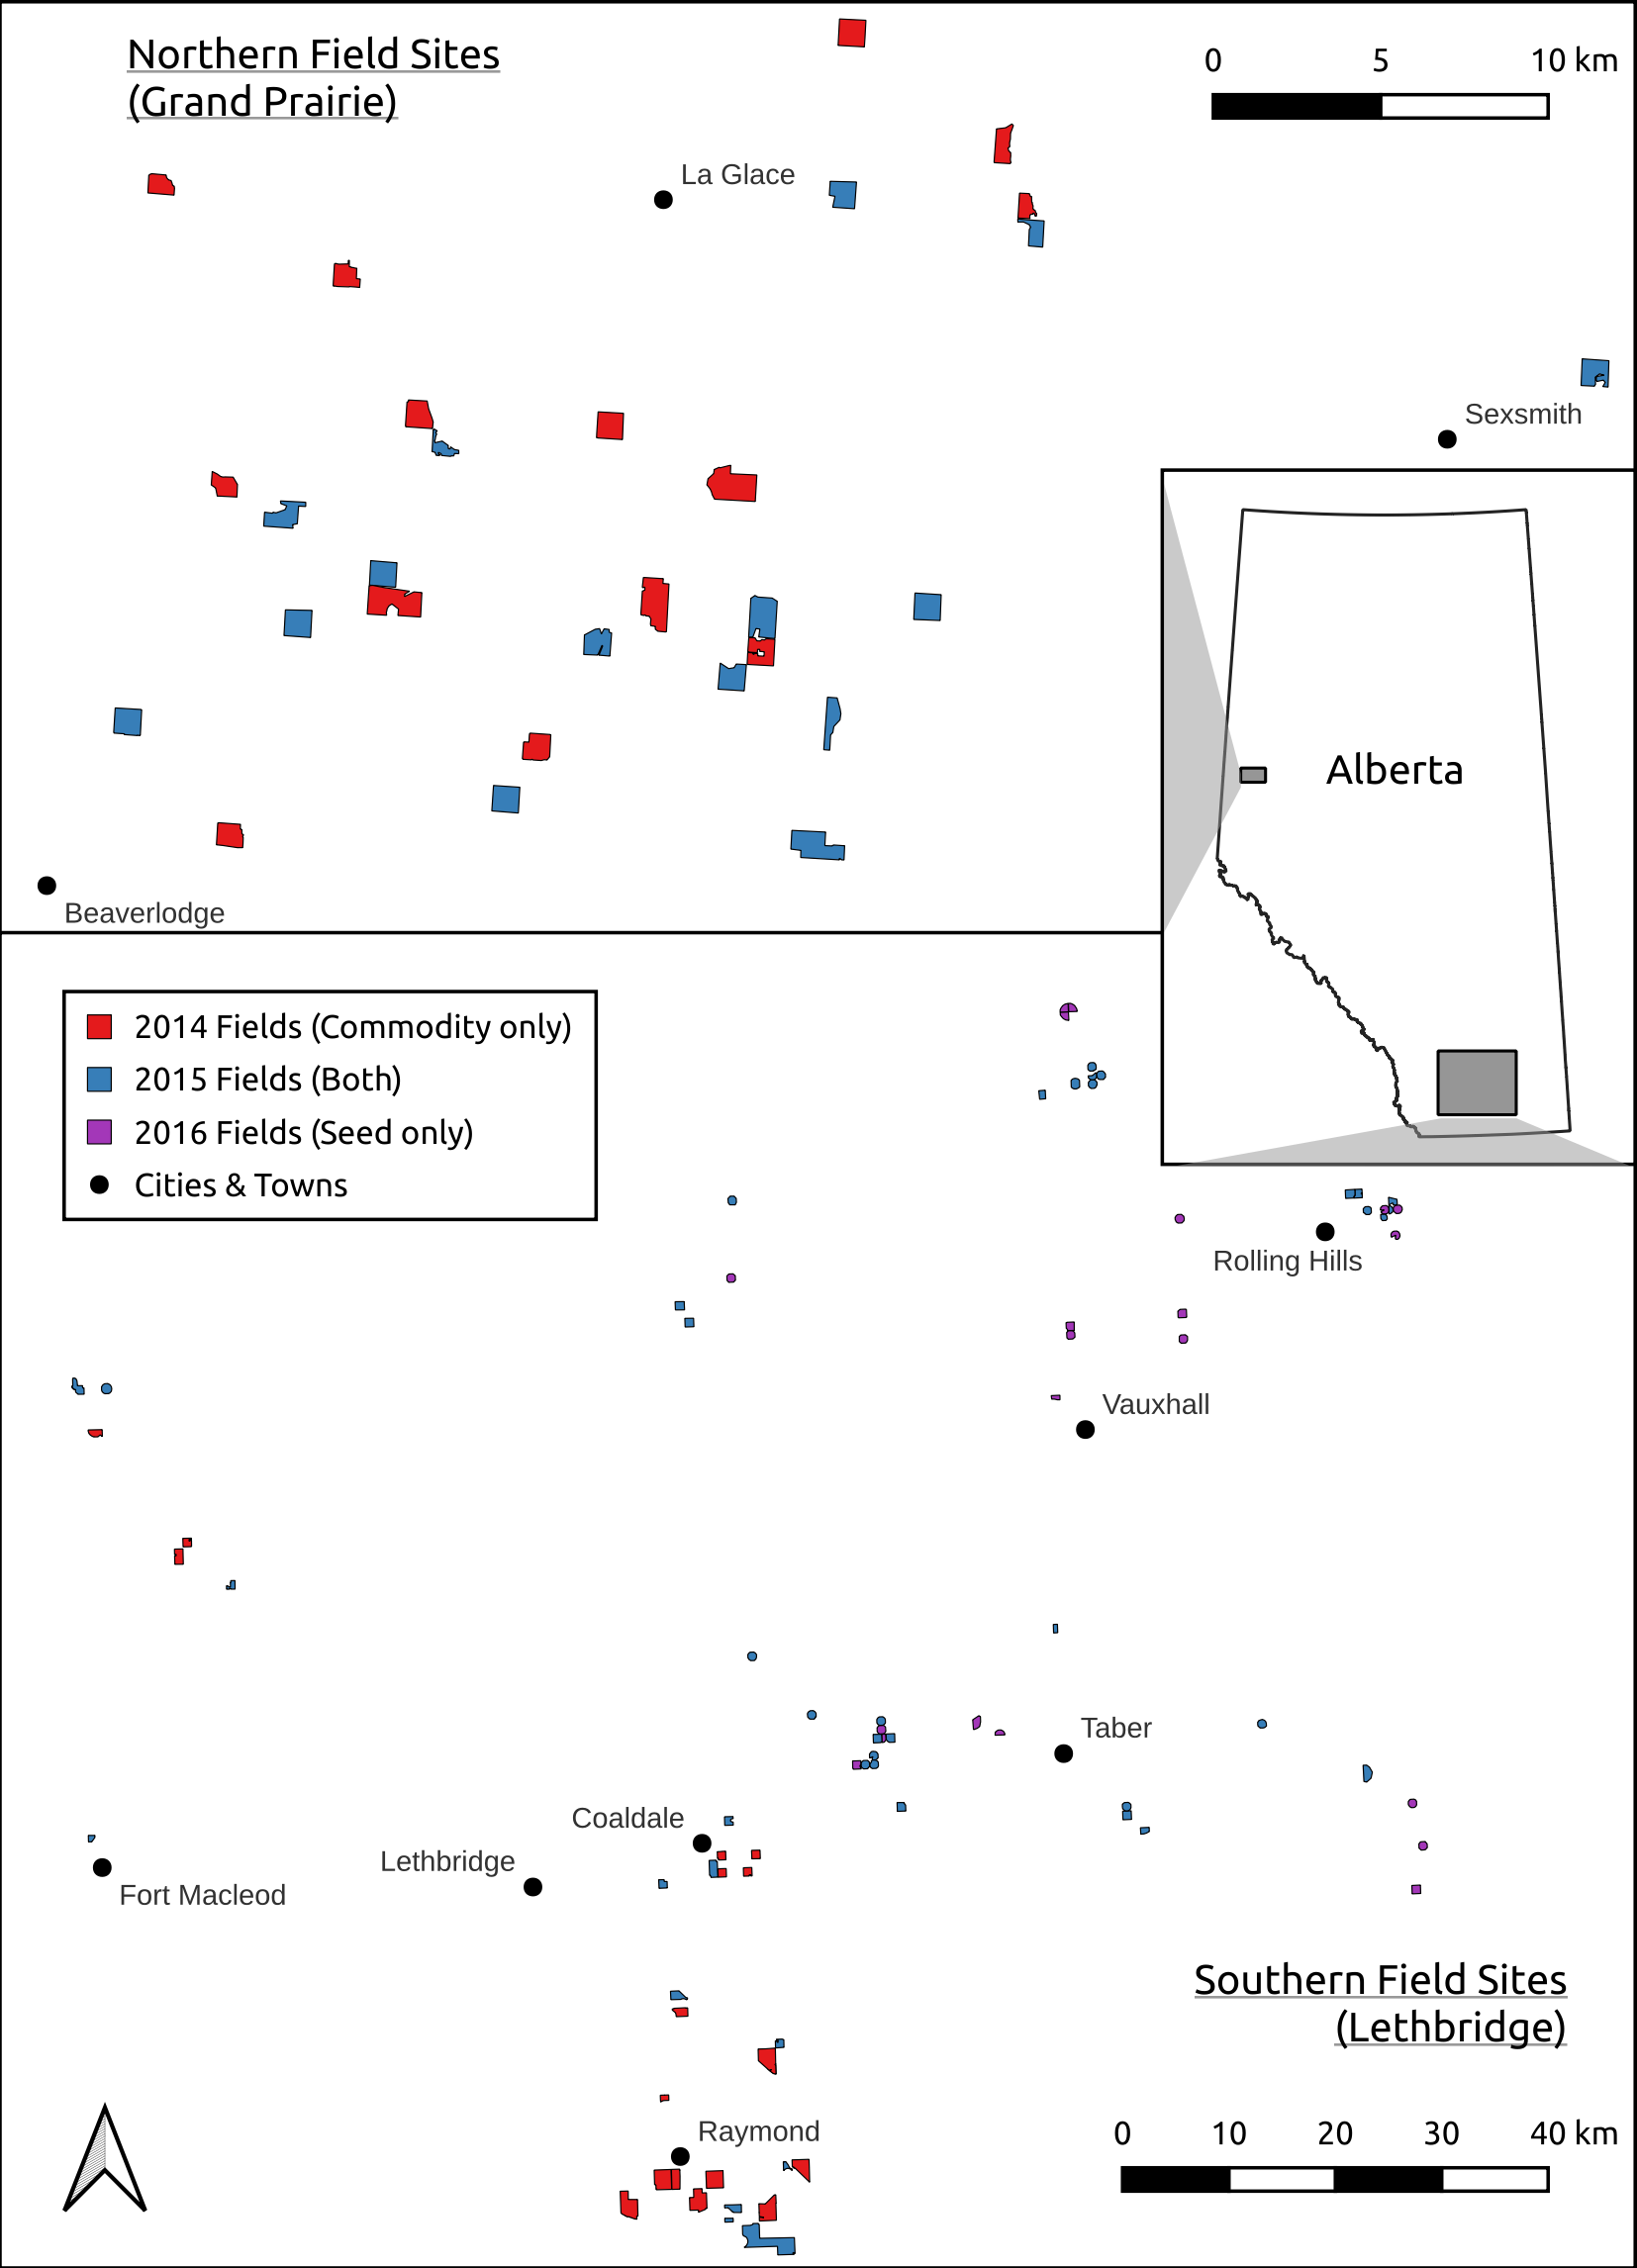
\includegraphics[width=\textwidth,keepaspectratio=true]{../Figures/FieldLocations.png}
    \caption{Map of sampled fields, showing locations of 29 commodity canola fields (14 during 2014, 15 during 2015), and 35 seed canola fields (15 during 2015, 20 during 2016). Seed canola is grown only in southern Alberta, while commodity canola is grown across both the northern and southern regions.}
    \label{fig:fieldMap}
\end{figure}


\begin{figure}
    \centering
    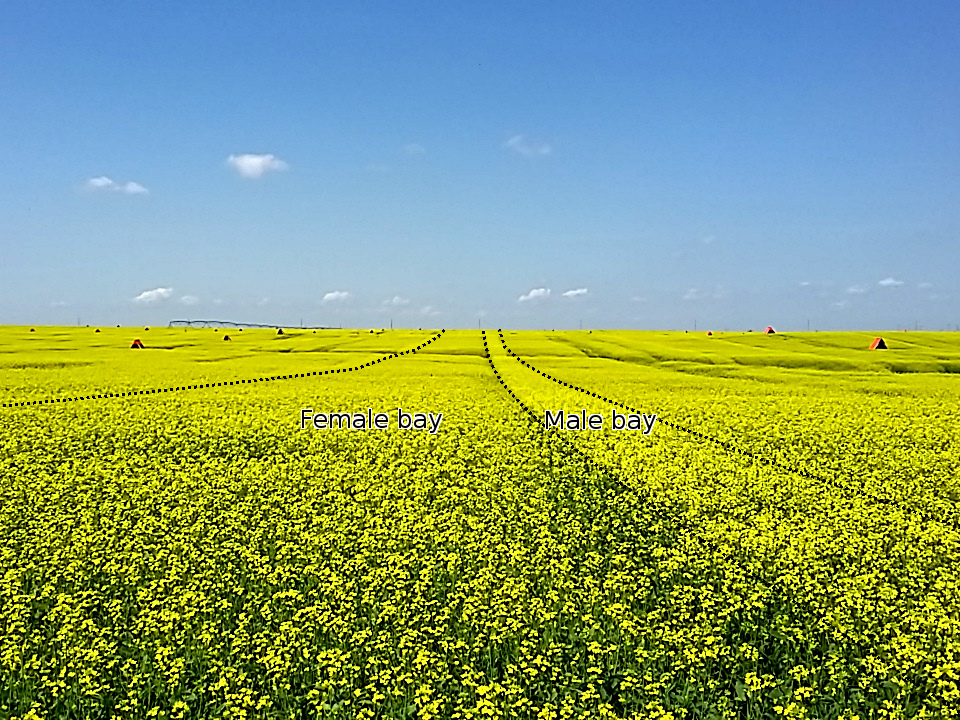
\includegraphics[width=\textwidth,keepaspectratio=true]{seedfieldBays.jpg}
    \caption[Hybrid seed field near Rainer, AB]{Hybrid seed field near Rainer, AB, showing the outlines of male and female bays in the foreground, with orange leafcutter bee shelters stationed throughout the field. The linear structure on the horizon is the central-pivot irrigation sprinkler.}
    \label{fig:seedfieldPhoto}
\end{figure}

\begin{figure}
    \centering
    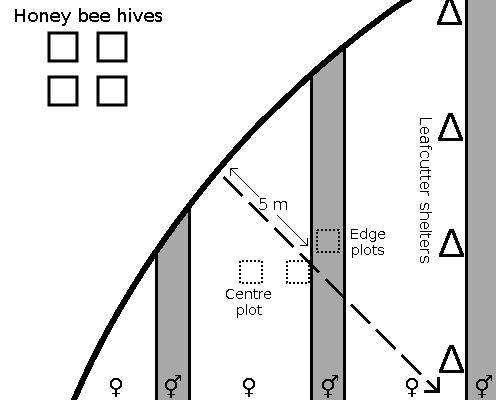
\includegraphics[width=0.6\textwidth,keepaspectratio=true]{seedfieldPlots.png}
    \caption[Plot arrangement for surveys in hybrid seed fields]{Plot arrangement for surveys in hybrid seed fields, showing hypothetical arrangement of leafcutter shelters ($\Delta$), and male-fertile (\Hermaphrodite) and female bays (\Female) at 5m from the edge of the field. Plots were placed 5, 20, 100, and 400m along a transect (dashed line) from the field edge nearest to the set of honey bee hives. Plots were placed side-by-side in the male bay and edge of the female bay (``edge" plots), and at the 5m and 400m distances, a plot was placed in the centre of the female bay (``centre" plots).}
    \label{fig:seedfieldPlots}
\end{figure}

\begin{table}
\caption{Summary of variables used in structural equation models.}
\centering

\begin{tabular}{l|l|r|r|r|r|r}
\hline
Field Type & Variable & Mean & Median & SD & Min & Max\\
\hline
 & Number of hives & 14.80 & 0.00 & 17.03 & 0.00 & 40.00\\
\cline{2-7}
 & Distance to edge (m) & 137.48 & 20.00 & 195.02 & 1.00 & 500.00\\
\cline{2-7}
 & HB visitation (hr$^{-1}$) & 10.31 & 0.00 & 28.80 & 0.00 & 218.18\\
\cline{2-7}
 & Flower density (m$^2$) & 470.33 & 448.00 & 231.32 & 52.00 & 1684.00\\
\cline{2-7}
 & Pollen per stigma & 293.33 & 155.00 & 385.04 & 0.00 & 3891.00\\
\cline{2-7}
 & Plant density (m$^2$) & 3.77 & 3.77 & 0.48 & 1.79 & 5.02\\
\cline{2-7}
 & Plant vegetative mass (g) & 18.15 & 14.32 & 14.07 & 0.77 & 107.66\\
\cline{2-7}
 & Plant seed mass (g) & 6.87 & 5.46 & 5.97 & 0.01 & 47.90\\
\cline{2-7}
 & Harvest index (g/g) & 0.38 & 0.37 & 0.16 & 0.00 & 1.89\\
\cline{2-7}
 & Flowers per plant & 196.09 & 156.50 & 150.96 & 13.00 & 1094.00\\
\cline{2-7}
 & Pods per plant & 143.15 & 112.00 & 114.64 & 5.00 & 892.00\\
\cline{2-7}
 & Seeds per pod & 22.96 & 23.60 & 4.97 & 4.60 & 35.40\\
\cline{2-7}
\multirow{-13}{*}{\raggedright\arraybackslash Commodity} & Seed size (mg) & 2.74 & 2.73 & 0.80 & 0.39 & 5.35\\
\cline{1-7}
 & Distance to edge (m) & 162.70 & 100.00 & 146.18 & 3.00 & 400.00\\
\cline{2-7}
 & Distance to LCB shelter (m) & 33.51 & 31.00 & 24.63 & 2.00 & 190.00\\
\cline{2-7}
 & HB visitation (hr$^{-1}$) & 112.79 & 24.00 & 187.30 & 0.00 & 1290.00\\
\cline{2-7}
 & LCB visitation (hr$^{-1}$) & 76.15 & 12.00 & 144.88 & 0.00 & 1272.00\\
\cline{2-7}
 & Bay Edge/Centre & 0.13 & 0.00 & 0.34 & 0.00 & 1.00\\
\cline{2-7}
 & Flower density (m$^2$) & 495.02 & 432.00 & 303.35 & 24.00 & 2686.40\\
\cline{2-7}
 & Pollen per stigma & 21.76 & 7.00 & 42.53 & 0.00 & 578.00\\
\cline{2-7}
 & Plant density (m$^2$) & 3.58 & 3.64 & 0.46 & 2.40 & 4.49\\
\cline{2-7}
 & Plant vegetative mass (g) & 30.32 & 25.19 & 21.16 & 1.18 & 144.32\\
\cline{2-7}
 & Plant seed mass (g) & 9.50 & 7.54 & 7.90 & 0.02 & 60.77\\
\cline{2-7}
 & Harvest index (g/g) & 0.32 & 0.33 & 0.15 & 0.00 & 1.21\\
\cline{2-7}
 & Flowers per plant & 461.32 & 362.50 & 326.59 & 26.00 & 2712.00\\
\cline{2-7}
 & Pods per plant & 299.41 & 244.50 & 207.68 & 10.00 & 1410.00\\
\cline{2-7}
 & Seeds per pod & 16.40 & 16.60 & 5.52 & 1.80 & 30.60\\
\cline{2-7}
\multirow{-15}{*}{\raggedright\arraybackslash Seed} & Seed size (mg) & 3.43 & 3.42 & 0.88 & 1.04 & 5.59\\
\hline
\end{tabular}

\label{tab:dataSummary}
\end{table}

\clearpage

\section*{Appendix B: Additional information on insect visitors}

\newline

During 2015, we recorded whether honey bees were top-working or side-working flowers (see also \citealp{free1973, free1983, mohr1988}).
Top-working bees landed on the top of the flower and inserted their proboscis down between the petals to access the nectaries of the flower, while side-working bees landed on the side of the flower and stole nectar by inserted their proboscis between the petals, avoiding contact with the stigma or anthers. 
Additionally, we recorded whether honey bees were pollen or nectar foragers (pollen foragers had a visible pollen load on their corbicula, while nectar foragers had none).

Pollen- and nectar-foraging honey bees had different patterns of side-working, both on commodity canola, and the male and female lines of seed canola.
Side-working was common in nectar foragers, but was more common in commodity canola (64\%) than in the male (36\%) or female bays (2.8\%) of seed canola, indicating that a large proportion of honey bees foraging on canola flowers may never come in contact with the stigmas.
Pollen foragers were almost uniformly top-foragers in both commodity and seed fields (Table \ref{tab:sideWorking}), and pollen foragers were much less common in the female bays (1.4\%) than in the male bays (15\%), or in commodity fields (18\%).
Therefore, foraging honey bees in seed canola fields tend to treat male-fertile flowers similar to commodity canola flowers, but seem to top-work flowers more in commodity canola than seed fields.
Leafcutter bee foraging behaviours were not recorded, but seemed to almost exclusively top-work flowers in seed canola fields.

\begin{table}
    \begin{tabular}{r|r|l|r|l}
     & \multicolumn{2}{c|}{Commodity fields} & \multicolumn{2}{c}{Seed fields} \\ \cline{2-5}
    Taxon & Visits & \% & Visits & \% \\ \hline
    Honey bee & 470 & 53.5 & 4850 & 77.1 \\
    Fly & 222 & 25.3 & 74 & 0.878 \\
    Hover fly & 94 & 10.7 & 151 & 1.79 \\
    Other bee & 47 & 5.35 & 30 & 0.356 \\
    Bumble bee & 25 & 2.85 & 0 & 0 \\
    Butterfly & 16 & 1.82 & 0 & 0 \\
    Leafcutter bee & 4 & 0.456 & 1675 & 19.9 \\
    % \hline
    % Total & 828 & - & 6780 & - \\
    \end{tabular}
    \caption{Number of flower visitors recorded over a total of 44.8 hours of observation in commodity fields (2014 and 2015), and 46.9 hours of observation in the seed fields (2015 and 2016). ``Fly" refers to larger calyptrate muscoid flies (families Muscidae, Anthomyiidae, Caliphoridae), while ``Hover fly" refers to Syrphid flies. ``Other bee" included Halictid and Andrenid bees, while ``Bumble bee" was \textit{Bombus} spp. ``Butterfly" refers to all visiting Lepidopterans, mostly Pierids.}
    \label{tab:propVisitors}  
\end{table}

\begin{table}
\begin{tabular}{r|r|l|r|l|r|l}
               & \multicolumn{2}{c|}{Commodity fields} & \multicolumn{2}{c|}{Seed fields (female bay)} & \multicolumn{2}{c}{Seed fields (male bay)} \\ \cline{2-7}
               & Top & Side & Top & Side & Top & Side           \\ \hline
Pollen forager & 44 & 2 & 12 & 0 & 115 & 0 \\
Nectar forager & 75 & 138 & 832 & 24 & 428 & 242 \\
% Total & 119 & 140 & 844 & 24 & 543 & 242
\end{tabular}
\caption[Foraging behaviours of honey bees on commodity and seed canola flowers]{Foraging behaviours of honey bees on commodity and seed canola flowers, recorded during 2015. ``Top" (top-working) indicates that the bee inserted their proboscis down between the petals from the top of the flower, while ``side" (side-working) indicates that the bee fed from the side of the flower and did not contact the anthers or stigma. Pollen foragers had pollen visible on their corbicula, while nectar foragers had none.}
\label{tab:sideWorking}
\end{table}

\clearpage

\section*{Appendix C: Additional information on models}

\subsection*{Commodity canola models}

Formulas for commodity canola model using \texttt{lmer}-style R formulas. Terms on right side of $\sim$ indicate fixed effects, while terms in brackets indicate random effects (heirarchical intercepts). \textit{distribution} indicates the type of probability distribution function used to model each variable.

\begin{align*}
    \text{Plant Density} \sim & \text{HB Distance} + (1|\text{Field}), \text{distribution = log-normal} \\
    \text{Plant Size} \sim & \text{Plant Density} + \text{HB Distance} + (1|\text{Field}),\text{distribution = log-normal} \\
    \text{Flower Density} \sim & \text{Plant Size} + \text{HB Distance} + \text{Plant Density} + (1|\text{Field}),\\
    &   \text{distribution = square root-normal} \\
    \text{HB Visits} \sim & \text{offset}(log(\text{Time})) + \text{HB Distance} + \text{Hive Stocking} + \\ 
    &   \text{Flower Density} + (1|\text{Field}), \text{family = negative binomial}\\
    \text{Pollen per Stigma} \sim & \text{HB Visits} + \text{HB Distance} + (1|\text{Field}), \text{distribution = negative binomial} \\
    \text{Flowers per Plant} \sim & \text{Plant Size} + \text{\% Pod Set} + (1|\text{Field}), \phi \sim \text{Plant Size}, \\
    &     \text{distribution = negative binomial} \\
    \text{\% Pod Set} \sim & \text{HB Visits} + \text{Pollen} + \text{Plant Size} + (1|\text{Field}), \text{distribution = beta-binomial} \\
    \text{Seeds per Pod} \sim & \text{HB Visits} + \text{Pollen} + \text{Plant Size} + \text{\% Pod Set} + \text{Flowers per Plant} + (1|\text{Field}),\\ 
    &   \text{distribution = exponential-normal} \\
    \text{Weight per Seed} \sim & \text{HB Visits} + \text{Pollen} + \text{Seeds per Pod} + \text{Plant Size} + \text{Plant Density} +\\
    &   \text{HB Distance} + \text{\% Pod Set} + \text{Flowers per Plant} + \text{Flower Density} + (1|\text{Field}),\\
    &   \text{distribution = exponential-normal} \\
\end{align*}

\begingroup\fontsize{9}{11}\selectfont

\begin{longtable}{l|l|r|r|r|r|r|l|r|r}

\caption{Summary of parameters for commodity canola models} \\

\hline
Model & Parameter & Mean & SD & Median & Min & Max & P-value & N$_{eff}$ & $\hat{R}$\\
\hline
\endfirsthead
\multicolumn{10}{@{}l}{\textit{(continued)}}\\
\hline
Model & Parameter & Mean & SD & Median & Min & Max & P-value & N$_{eff}$ & $\hat{R}$\\
\hline
\endhead
 & Intercept & 3.76 & 0.05 & 3.77 & 3.66 & 3.87 & $<$0.0001 & 855 & 1.005\\
\cline{2-10}
 & HB distance & 0.02 & 0.01 & 0.02 & 0.00 & 0.04 & 0.0868 & 10154 & 1.000\\
\cline{2-10}
 & Sigma & 0.31 & 0.02 & 0.31 & 0.28 & 0.34 & - & 5039 & 0.999\\
\cline{2-10}
\multirow{-4}{*}{\raggedright\arraybackslash Plant density} & Sigma (field) & 0.37 & 0.04 & 0.37 & 0.30 & 0.46 & - & 3774 & 1.000\\
\cline{1-10}
 & Intercept & 5.24 & 0.24 & 5.24 & 4.77 & 5.72 & $<$0.0001 & 2108 & 1.001\\
\cline{2-10}
 & Plant density & -0.70 & 0.06 & -0.70 & -0.82 & -0.57 & $<$0.0001 & 2097 & 1.001\\
\cline{2-10}
 & HB distance & 0.03 & 0.01 & 0.03 & 0.01 & 0.06 & 0.0095 & 9212 & 1.000\\
\cline{2-10}
 & Sigma (field) & 0.22 & 0.04 & 0.22 & 0.15 & 0.29 & - & 1456 & 1.000\\
\cline{2-10}
\multirow{-5}{*}{\raggedright\arraybackslash Plant size} & Sigma & 0.64 & 0.02 & 0.64 & 0.61 & 0.68 & - & 7845 & 0.999\\
\cline{1-10}
 & Intercept & 5.74 & 4.70 & 5.70 & -3.62 & 15.01 & 0.222 & 1822 & 1.001\\
\cline{2-10}
 & Plant size & -1.66 & 0.98 & -1.66 & -3.60 & 0.25 & 0.0926 & 1632 & 1.001\\
\cline{2-10}
 & HB distance & 0.75 & 0.11 & 0.75 & 0.53 & 0.96 & $<$0.0001 & 6878 & 1.000\\
\cline{2-10}
 & Plant density & -0.41 & 0.74 & -0.42 & -1.86 & 1.06 & 0.5792 & 2243 & 1.001\\
\cline{2-10}
 & Sigma & 3.52 & 0.17 & 3.51 & 3.19 & 3.87 & - & 4976 & 0.999\\
\cline{2-10}
\multirow{-6}{*}{\raggedright\arraybackslash Flower density} & Sigma (field) & 3.55 & 0.39 & 3.53 & 2.88 & 4.40 & - & 4133 & 1.000\\
\cline{1-10}
 & Intercept & -1.98 & 0.45 & -1.96 & -2.89 & -1.17 & $<$0.0001 & 936 & 1.006\\
\cline{2-10}
 & HB distance & -0.31 & 0.10 & -0.31 & -0.50 & -0.13 & 0.0011 & 3526 & 1.001\\
\cline{2-10}
 & Number of hives & 0.72 & 0.15 & 0.72 & 0.43 & 1.04 & $<$0.0001 & 1534 & 1.003\\
\cline{2-10}
 & Flower density & 0.03 & 0.04 & 0.03 & -0.06 & 0.12 & 0.541 & 2397 & 1.000\\
\cline{2-10}
 & Sigma (field) & 1.44 & 0.34 & 1.43 & 0.80 & 2.14 & - & 494 & 1.014\\
\cline{2-10}
\multirow{-6}{*}{\raggedright\arraybackslash HB visits} & Phi & 0.35 & 0.08 & 0.34 & 0.22 & 0.53 & - & 1630 & 1.003\\
\cline{1-10}
 & Intercept & 2.56 & 0.04 & 2.56 & 2.50 & 2.63 & $<$0.0001 & 594 & 1.006\\
\cline{2-10}
 & Plant size & 0.94 & 0.01 & 0.94 & 0.92 & 0.96 & $<$0.0001 & 1709 & 1.002\\
\cline{2-10}
 & Pods per plant & -0.16 & 0.01 & -0.16 & -0.19 & -0.14 & $<$0.0001 & 2108 & 1.003\\
\cline{2-10}
 & Phi (field) & 0.16 & 0.02 & 0.16 & 0.13 & 0.19 & - & 3461 & 1.000\\
\cline{2-10}
 & Intercept (Phi) & 2.17 & 0.32 & 2.17 & 1.56 & 2.81 & - & 1517 & 1.001\\
\cline{2-10}
 & Plant size (Phi) & 0.66 & 0.11 & 0.66 & 0.44 & 0.87 & - & 1587 & 1.002\\
\cline{2-10}
\multirow{-7}{*}{\raggedright\arraybackslash Flowers per plant} & SigmaPhi (field) & 0.66 & 0.12 & 0.65 & 0.45 & 0.90 & - & 844 & 1.005\\
\cline{1-10}
 & Intercept & 0.66 & 0.08 & 0.66 & 0.50 & 0.82 & $<$0.0001 & 1946 & 0.999\\
\cline{2-10}
 & HB visits & 0.00 & 0.03 & 0.00 & -0.05 & 0.05 & 0.96 & 3292 & 1.000\\
\cline{2-10}
 & Plant size & 0.13 & 0.03 & 0.13 & 0.08 & 0.18 & $<$0.0001 & 3345 & 1.000\\
\cline{2-10}
 & Pollen count & 0.16 & 0.11 & 0.15 & -0.05 & 0.38 & 0.1515 & 638 & 1.002\\
\cline{2-10}
 & Sigma (field) & 0.29 & 0.03 & 0.29 & 0.23 & 0.37 & - & 2675 & 1.000\\
\cline{2-10}
\multirow{-6}{*}{\raggedright\arraybackslash Pods per plant} & Phi & 3.35 & 0.07 & 3.35 & 3.21 & 3.48 & - & 3828 & 1.003\\
\cline{1-10}
 & Intercept & 25.07 & 1.77 & 25.07 & 21.64 & 28.54 & $<$0.0001 & 2277 & 1.000\\
\cline{2-10}
 & HB visits & 0.17 & 0.21 & 0.17 & -0.24 & 0.60 & 0.4284 & 4417 & 1.000\\
\cline{2-10}
 & Pollen count & -0.97 & 0.84 & -0.98 & -2.60 & 0.68 & 0.2447 & 707 & 1.003\\
\cline{2-10}
 & Plant size & 4.31 & 0.65 & 4.31 & 3.03 & 5.58 & $<$0.0001 & 2229 & 1.000\\
\cline{2-10}
 & Pods per plant & 0.56 & 0.29 & 0.56 & 0.00 & 1.12 & 0.0529 & 4888 & 0.999\\
\cline{2-10}
 & Flowers per plant & -2.80 & 0.65 & -2.79 & -4.08 & -1.55 & $<$0.0001 & 2105 & 1.000\\
\cline{2-10}
 & Sigma & 4.06 & 0.12 & 4.06 & 3.83 & 4.29 & - & 6604 & 1.000\\
\cline{2-10}
 & Sigma (field) & 1.98 & 0.26 & 1.96 & 1.51 & 2.53 & - & 2526 & 0.999\\
\cline{2-10}
\multirow{-9}{*}{\raggedright\arraybackslash Seeds per pod} & Lambda & 2.00 & 1.03 & 1.74 & 0.84 & 4.64 & - & 3265 & 1.000\\
\cline{1-10}
 & Intercept & 0.64 & 0.54 & 0.64 & -0.40 & 1.72 & 0.2367 & 1402 & 1.000\\
\cline{2-10}
 & HB visits & 0.02 & 0.04 & 0.02 & -0.05 & 0.09 & 0.6113 & 2748 & 1.000\\
\cline{2-10}
 & Pollen count & -0.15 & 0.17 & -0.15 & -0.48 & 0.20 & 0.3744 & 358 & 1.008\\
\cline{2-10}
 & Seeds per pod & 0.00 & 0.01 & 0.00 & -0.01 & 0.02 & 0.4508 & 3348 & 1.000\\
\cline{2-10}
 & Plant size & -0.03 & 0.12 & -0.03 & -0.26 & 0.20 & 0.7955 & 1633 & 1.000\\
\cline{2-10}
 & Plant density & 0.30 & 0.08 & 0.30 & 0.14 & 0.45 & 0.0001 & 1704 & 1.001\\
\cline{2-10}
 & HB distance & 0.02 & 0.01 & 0.02 & -0.01 & 0.05 & 0.1686 & 1404 & 1.003\\
\cline{2-10}
 & Pods per plant & 0.11 & 0.04 & 0.11 & 0.02 & 0.19 & 0.0159 & 3037 & 1.000\\
\cline{2-10}
 & Flowers per plant & 0.11 & 0.12 & 0.11 & -0.13 & 0.34 & 0.363 & 1526 & 1.000\\
\cline{2-10}
 & Flower density & -0.03 & 0.01 & -0.03 & -0.04 & -0.02 & $<$0.0001 & 2213 & 1.003\\
\cline{2-10}
 & Sigma & 0.52 & 0.03 & 0.52 & 0.46 & 0.59 & - & 2100 & 1.000\\
\cline{2-10}
 & Sigma (field) & 0.47 & 0.05 & 0.47 & 0.37 & 0.58 & - & 2828 & 0.999\\
\cline{2-10}
\multirow{-13}{*}{\raggedright\arraybackslash Seed size} & Lambda & 2.71 & 0.48 & 2.63 & 2.08 & 3.86 & - & 1792 & 1.001\\
\hline
\label{tab:commCoefs}
\end{longtable}
\endgroup{}

\subsection*{Seed canola models}

Formulas for seed canola model using \texttt{lmer}-style R formulas. Terms on right side of $\sim$ indicate fixed effects, while terms in brackets indicate random effects (heirarchical intercepts). \textit{distribution} indicates the type of probability distribution function used to model each variable.

\begin{align*}
    \text{Plant Density} \sim & \text{HB Distance} + (1|\text{Field}), \text{distribution = log-normal} \\
    \text{Plant Size} \sim & \text{HB Distance} + \text{Plant Density} + (1|\text{Field}) ,\text{distribution = log-t} \\
    \text{Flower Density} \sim & \text{HB Distance} + (1|\text{Field}), \text{distribution = square root-t} \\
    \text{LCB Visits} \sim & \text{offset}(log(\text{Time})) + \text{HB Distance} + \text{LCB Distance} + \text{Bay Centre} + \\
    &   \text{Flower Density} + (1|\text{Field}), \text{family = ZI negative binomial} \\
    \text{HB Visits} \sim & \text{offset}(log(\text{Time})) + \text{HB Distance} + \text{LCB Distance} + \text{Bay Centre} + \\
    &   \text{Flower Density} + (1|\text{Field}), \text{family = ZI negative binomial} \\
    \text{Pollen per Stigma} \sim & \text{HB Visits} + \text{LCB Visits} + \text{Bay Centre} + \text{HB Distance} + \text{LCB Distance} +\\
    &   \text{Flower Density} + (1|\text{Field}) + (1|\text{Plot}), \text{family = negative binomial} \\
    \text{Flowers per Plant} \sim & \text{Plant Size} + \text{Bay Centre} + \text{\% Pod Set} + (1|\text{Field}),\\
    &   \phi \sim \text{Plant Size}, \text{family = negative binomial} \\
    \text{\% Pod Set} \sim & \text{Pollen} + \text{Plant Size} + \text{Bay Centre} + \text{HB Distance} + \text{LCB Distance} + \\
    &   \text{Flower Density} + (1|\text{Field}) + (1|\text{Plot}), \text{family = beta-binomial} \\
    \text{Seeds per Pod} \sim & \text{Pollen} + \text{Plant Size} + \text{Bay Centre} + \text{HB Distance} + \text{Flower Density} +\\
    &   \text{\% Pod Set} + \text{Flowers per plant} + (1|\text{Field}), \text{family = negative binomial} \\
    \text{Weight per Seed} \sim & \text{Pollen} + \text{Seeds per Pod} + \text{Plant Size} + \text{LCB Distance} +\\
    &   \text{Plant Density} + (1|\text{Field}), \text{family = exponential-normal}\\
\end{align*}


\begingroup\fontsize{9}{11}\selectfont

\begin{longtable}{l|l|r|r|r|r|r|l|r|r}

\caption{Summary of parameters for seed canola models} \\

\hline
Model & Parameter & Mean & SD & Median & Min & Max & P-value & N$_{eff}$ & $\hat{R}$\\
\hline
\endfirsthead
\multicolumn{10}{@{}l}{\textit{(continued)}}\\
\hline
Model & Parameter & Mean & SD & Median & Min & Max & P-value & N$_{eff}$ & $\hat{R}$\\
\hline
\endhead
 & Intercept & 3.60 & 0.06 & 3.60 & 3.47 & 3.73 & $<$0.0001 & 524 & 1.004\\
\cline{2-10}
 & HB distance & 0.06 & 0.01 & 0.06 & 0.04 & 0.07 & $<$0.0001 & 5750 & 0.999\\
\cline{2-10}
 & Sigma & 0.27 & 0.01 & 0.27 & 0.24 & 0.30 & - & 5199 & 0.999\\
\cline{2-10}
\multirow{-4}{*}{\raggedright\arraybackslash Plant density} & Sigma (field) & 0.36 & 0.05 & 0.36 & 0.28 & 0.48 & - & 4182 & 1.000\\
\cline{1-10}
 & Intercept & 6.08 & 0.25 & 6.08 & 5.57 & 6.56 & $<$0.0001 & 2480 & 1.000\\
\cline{2-10}
 & Plant density & -0.79 & 0.07 & -0.80 & -0.92 & -0.66 & $<$0.0001 & 2470 & 1.000\\
\cline{2-10}
 & HB distance & 0.07 & 0.01 & 0.07 & 0.05 & 0.10 & $<$0.0001 & 6446 & 0.999\\
\cline{2-10}
 & Sigma & 0.50 & 0.03 & 0.50 & 0.45 & 0.56 & - & 2332 & 1.000\\
\cline{2-10}
 & Sigma (field) & 0.15 & 0.04 & 0.15 & 0.08 & 0.23 & - & 1053 & 1.001\\
\cline{2-10}
\multirow{-6}{*}{\raggedright\arraybackslash Plant size} & Nu (DF) & 1.91 & 0.32 & 1.87 & 1.37 & 2.65 & $<$0.0001 & 2700 & 1.000\\
\cline{1-10}
 & Intercept & 0.48 & 0.56 & 0.46 & -0.58 & 1.64 & 0.3827 & 661 & 1.005\\
\cline{2-10}
 & HB distance & 1.11 & 0.12 & 1.11 & 0.87 & 1.36 & $<$0.0001 & 5389 & 1.000\\
\cline{2-10}
 & Sigma & 4.06 & 0.24 & 4.05 & 3.59 & 4.56 & - & 2404 & 1.001\\
\cline{2-10}
 & Sigma (field) & 3.48 & 0.47 & 3.44 & 2.70 & 4.49 & - & 2640 & 1.001\\
\cline{2-10}
\multirow{-5}{*}{\raggedright\arraybackslash Flower density} & Nu (DF) & 1.88 & 0.38 & 1.84 & 1.30 & 2.68 & $<$0.0001 & 1500 & 1.004\\
\cline{1-10}
 & Intercept & 3.08 & 0.10 & 3.08 & 2.87 & 3.28 & $<$0.0001 & 2722 & 1.002\\
\cline{2-10}
 & Flower density & -0.01 & 0.01 & -0.01 & -0.03 & 0.01 & 0.5267 & 4150 & 1.000\\
\cline{2-10}
 & HB distance & -0.02 & 0.05 & -0.03 & -0.12 & 0.07 & 0.6229 & 4410 & 1.000\\
\cline{2-10}
 & LCB distance & 0.42 & 0.09 & 0.42 & 0.24 & 0.58 & $<$0.0001 & 5053 & 1.000\\
\cline{2-10}
 & Bay centre & 0.45 & 0.21 & 0.45 & 0.07 & 0.88 & 0.0284 & 6486 & 0.999\\
\cline{2-10}
 & Phi & 0.72 & 0.09 & 0.72 & 0.55 & 0.92 & - & 4354 & 1.001\\
\cline{2-10}
 & Theta (ZI) & 0.32 & 0.03 & 0.32 & 0.26 & 0.38 & - & 3955 & 1.001\\
\cline{2-10}
\multirow{-8}{*}{\raggedright\arraybackslash HB visits} & Sigma (field) & 0.41 & 0.11 & 0.41 & 0.22 & 0.64 & - & 600 & 1.001\\
\cline{1-10}
 & Intercept & 2.25 & 0.14 & 2.25 & 1.96 & 2.51 & $<$0.0001 & 1734 & 1.002\\
\cline{2-10}
 & LCB distance & -0.79 & 0.07 & -0.79 & -0.94 & -0.65 & $<$0.0001 & 4016 & 1.000\\
\cline{2-10}
 & HB distance & -0.32 & 0.06 & -0.32 & -0.43 & -0.21 & $<$0.0001 & 5128 & 1.000\\
\cline{2-10}
 & Bay centre & -0.34 & 0.23 & -0.34 & -0.77 & 0.16 & 0.1458 & 6667 & 1.000\\
\cline{2-10}
 & Flower density & 0.03 & 0.01 & 0.03 & 0.01 & 0.05 & 0.0115 & 4364 & 1.000\\
\cline{2-10}
 & Sigma (field) & 0.63 & 0.13 & 0.62 & 0.40 & 0.91 & - & 1072 & 1.004\\
\cline{2-10}
 & Phi & 0.70 & 0.11 & 0.69 & 0.50 & 0.93 & - & 3097 & 0.999\\
\cline{2-10}
\multirow{-8}{*}{\raggedright\arraybackslash LCB visits} & Theta (ZI) & 0.25 & 0.04 & 0.25 & 0.15 & 0.33 & - & 2383 & 1.000\\
\cline{1-10}
 & Intercept & 2.49 & 0.19 & 2.50 & 2.12 & 2.85 & $<$0.0001 & 1141 & 1.002\\
\cline{2-10}
 & HB visits & 0.05 & 0.04 & 0.05 & -0.03 & 0.12 & 0.195 & 2317 & 1.000\\
\cline{2-10}
 & LCB visits & 0.15 & 0.06 & 0.14 & 0.02 & 0.26 & 0.0155 & 2239 & 1.000\\
\cline{2-10}
 & Bay centre & -0.55 & 0.13 & -0.55 & -0.80 & -0.30 & $<$0.0001 & 2540 & 1.000\\
\cline{2-10}
 & HB distance & -0.17 & 0.04 & -0.17 & -0.25 & -0.09 & $<$0.0001 & 2265 & 1.003\\
\cline{2-10}
 & LCB distance & -0.35 & 0.14 & -0.35 & -0.63 & -0.07 & 0.0164 & 2513 & 1.000\\
\cline{2-10}
 & Flower density & -0.03 & 0.02 & -0.03 & -0.06 & 0.01 & 0.1284 & 2058 & 1.001\\
\cline{2-10}
 & Sigma (field) & 0.86 & 0.13 & 0.85 & 0.64 & 1.15 & - & 2978 & 1.000\\
\cline{2-10}
 & Sigma (plot) & 0.65 & 0.06 & 0.65 & 0.53 & 0.78 & - & 1142 & 1.003\\
\cline{2-10}
\multirow{-10}{*}{\raggedright\arraybackslash Pollen count} & Phi & 0.82 & 0.04 & 0.82 & 0.74 & 0.90 & - & 5125 & 0.999\\
\cline{1-10}
 & Intercept & 3.05 & 0.04 & 3.05 & 2.96 & 3.14 & $<$0.0001 & 3283 & 0.999\\
\cline{2-10}
 & Plant size & 0.93 & 0.01 & 0.93 & 0.90 & 0.95 & $<$0.0001 & 3712 & 0.999\\
\cline{2-10}
 & Bay centre & 0.09 & 0.02 & 0.09 & 0.06 & 0.12 & $<$0.0001 & 6790 & 0.999\\
\cline{2-10}
 & Pods per plant & -0.14 & 0.01 & -0.14 & -0.17 & -0.12 & $<$0.0001 & 5503 & 0.999\\
\cline{2-10}
 & Sigma (field) & 0.08 & 0.01 & 0.08 & 0.06 & 0.11 & - & 2649 & 1.000\\
\cline{2-10}
 & Intercept (Phi) & 2.24 & 0.32 & 2.24 & 1.62 & 2.87 & - & 2875 & 1.001\\
\cline{2-10}
\multirow{-7}{*}{\raggedright\arraybackslash Flowers per plant} & Plant size (Phi) & 0.38 & 0.10 & 0.39 & 0.19 & 0.57 & - & 2871 & 1.001\\
\cline{1-10}
 & Intercept & 0.18 & 0.12 & 0.18 & -0.05 & 0.40 & 0.1211 & 2261 & 1.000\\
\cline{2-10}
 & Pollen count & 0.12 & 0.04 & 0.12 & 0.03 & 0.20 & 0.0074 & 915 & 1.004\\
\cline{2-10}
 & Plant size & 0.19 & 0.03 & 0.19 & 0.14 & 0.24 & $<$0.0001 & 4570 & 1.000\\
\cline{2-10}
 & Bay centre & -0.21 & 0.06 & -0.21 & -0.33 & -0.10 & 0.0003 & 1886 & 1.000\\
\cline{2-10}
 & HB distance & -0.12 & 0.02 & -0.12 & -0.15 & -0.08 & $<$0.0001 & 1929 & 1.002\\
\cline{2-10}
 & LCB distance & -0.21 & 0.06 & -0.21 & -0.34 & -0.10 & 0.0005 & 2637 & 1.000\\
\cline{2-10}
 & Flower density & 0.00 & 0.01 & 0.00 & -0.02 & 0.01 & 0.5456 & 2998 & 1.000\\
\cline{2-10}
 & Sigma (plot) & 0.30 & 0.03 & 0.30 & 0.25 & 0.35 & - & 1367 & 1.004\\
\cline{2-10}
 & Sigma (field) & 0.37 & 0.06 & 0.36 & 0.27 & 0.49 & - & 2905 & 1.000\\
\cline{2-10}
 & Intercept (Phi) & 3.07 & 0.38 & 3.05 & 2.36 & 3.85 & - & 2268 & 1.004\\
\cline{2-10}
\multirow{-11}{*}{\raggedright\arraybackslash Pods per plant} & Plant size (Phi) & 0.22 & 0.12 & 0.22 & -0.01 & 0.44 & - & 2538 & 1.003\\
\cline{1-10}
 & Intercept & 25.38 & 2.29 & 25.48 & 20.64 & 29.38 & $<$0.0001 & 1651 & 1.001\\
\cline{2-10}
 & Pollen count & 1.21 & 0.32 & 1.20 & 0.61 & 1.87 & 0.0001 & 1046 & 1.002\\
\cline{2-10}
 & Plant size & 4.76 & 0.78 & 4.76 & 3.24 & 6.23 & $<$0.0001 & 1752 & 1.001\\
\cline{2-10}
 & Bay centre & -0.50 & 0.45 & -0.50 & -1.39 & 0.38 & 0.2639 & 5315 & 0.999\\
\cline{2-10}
 & HB distance & -0.02 & 0.12 & -0.01 & -0.25 & 0.21 & 0.881 & 3007 & 1.000\\
\cline{2-10}
 & Flower density & -0.11 & 0.06 & -0.11 & -0.23 & 0.00 & 0.0451 & 2596 & 1.000\\
\cline{2-10}
 & Pods per plant & 1.65 & 0.35 & 1.65 & 0.94 & 2.34 & $<$0.0001 & 2485 & 1.001\\
\cline{2-10}
 & Flowers per plant & -4.26 & 0.74 & -4.27 & -5.60 & -2.73 & $<$0.0001 & 1571 & 1.001\\
\cline{2-10}
 & Sigma & 4.25 & 0.16 & 4.25 & 3.92 & 4.56 & - & 2951 & 1.000\\
\cline{2-10}
 & Sigma (field) & 1.97 & 0.32 & 1.95 & 1.41 & 2.68 & - & 1767 & 1.002\\
\cline{2-10}
\multirow{-11}{*}{\raggedright\arraybackslash Seeds per pod} & Lambda & 1.67 & 1.00 & 1.39 & 0.60 & 4.28 & - & 2448 & 0.999\\
\cline{1-10}
 & Intercept & 1.17 & 0.50 & 1.18 & 0.21 & 2.16 & 0.0189 & 2004 & 1.001\\
\cline{2-10}
 & Pollen count & -0.02 & 0.05 & -0.02 & -0.12 & 0.08 & 0.7002 & 2345 & 1.000\\
\cline{2-10}
 & Seeds per pod & -0.01 & 0.01 & -0.01 & -0.03 & 0.00 & 0.0765 & 3719 & 0.999\\
\cline{2-10}
 & Plant size & 0.23 & 0.06 & 0.23 & 0.12 & 0.34 & $<$0.0001 & 3607 & 1.000\\
\cline{2-10}
 & Plant density & 0.41 & 0.11 & 0.41 & 0.20 & 0.63 & 0.0002 & 1988 & 1.000\\
\cline{2-10}
 & LCB distance & 0.07 & 0.07 & 0.07 & -0.06 & 0.22 & 0.3146 & 4466 & 1.000\\
\cline{2-10}
 & Sigma & 0.75 & 0.03 & 0.75 & 0.69 & 0.81 & - & 3533 & 1.000\\
\cline{2-10}
 & Sigma (field) & 0.36 & 0.06 & 0.35 & 0.25 & 0.49 & - & 2060 & 1.000\\
\cline{2-10}
\multirow{-9}{*}{\raggedright\arraybackslash Seed size} & Lambda & 4.44 & 1.22 & 4.23 & 2.70 & 7.42 & - & 2125 & 1.000\\
\hline
\label{tab:seedCoefs}
\end{longtable}
\endgroup{}


\clearpage

\subsection*{Total yield models}

Formulas for total yield models are  using \texttt{lmer}-style R formulas. Predicted yield for each plant was calculated as: pods per plant $\times$ seeds per pod $\times$ weight per seed. Terms on right side of $\sim$ indicate fixed effects, while terms in brackets indicate random intercepts (and slopes). 

\begin{align*}
    \text{Total Yield} \sim & log(\text{Predicted Yield}) + (log(\text{Predicted Yield})|\text{Field}) + \\
    & (log(\text{Predicted Yield})|\text{Plot}), \text{distribution = log-normal} \\
\end{align*}

\begin{table}[h]
\centering\begingroup\fontsize{9}{11}\selectfont
\caption{Summary of parameters for total yield models}

\begin{tabular}{l|l|r|r|r|r|r|r|r|r|r}
\hline
Field Type & Parameter & Mean & SD & Z & median & Min & Max & p-value & N$_{eff}$ & $\hat{R}$\\
\hline
 & Intercept & -0.318 & 0.042 & -7.62 & -0.317 & -0.397 & -0.236 & 0.000 & 982 & 1.000\\
\cline{2-11}
 & Predicted Yield & 1.007 & 0.018 & 55.64 & 1.007 & 0.972 & 1.044 & 0.000 & 1044 & 1.000\\
\cline{2-11}
 & Sigma (field intercept) & 0.119 & 0.041 & 2.89 & 0.112 & 0.051 & 0.216 & 0.004 & 292 & 1.020\\
\cline{2-11}
 & Sigma (field slope) & 0.026 & 0.019 & 1.37 & 0.023 & 0.001 & 0.072 & 0.170 & 295 & 1.013\\
\cline{2-11}
 & Sigma (plot intercept) & 0.389 & 0.037 & 10.47 & 0.388 & 0.318 & 0.465 & 0.000 & 506 & 1.005\\
\cline{2-11}
 & Sigma (plot slope) & 0.169 & 0.017 & 9.86 & 0.168 & 0.135 & 0.204 & 0.000 & 556 & 1.006\\
\cline{2-11}
 & Sigma & 0.253 & 0.008 & 33.30 & 0.253 & 0.239 & 0.268 & 0.000 & 2002 & 1.000\\
\cline{2-11}
 & Correlation (Int:Slope field) & -0.400 & 0.448 & -0.89 & -0.525 & -0.944 & 0.626 & 0.372 & 660 & 1.005\\
\cline{2-11}
\multirow{-9}{*}{\raggedright\arraybackslash Commodity} & Correlation (Int:Slope plot) & -0.989 & 0.007 & -140.44 & -0.990 & -0.998 & -0.972 & 0.000 & 936 & 1.005\\
\cline{1-11}
 & Intercept & -0.210 & 0.072 & -2.90 & -0.210 & -0.348 & -0.066 & 0.004 & 738 & 1.007\\
\cline{2-11}
 & Predicted Yield & 0.856 & 0.025 & 34.62 & 0.856 & 0.806 & 0.904 & 0.000 & 672 & 1.008\\
\cline{2-11}
 & Sigma (field intercept) & 0.040 & 0.018 & 2.28 & 0.038 & 0.011 & 0.079 & 0.022 & 226 & 1.005\\
\cline{2-11}
 & Sigma (field slope) & 0.010 & 0.007 & 1.56 & 0.009 & 0.001 & 0.023 & 0.118 & 217 & 1.005\\
\cline{2-11}
 & Sigma (plot intercept) & 0.097 & 0.013 & 7.26 & 0.097 & 0.072 & 0.124 & 0.000 & 470 & 1.005\\
\cline{2-11}
 & Sigma (plot slope) & 0.032 & 0.005 & 5.83 & 0.032 & 0.021 & 0.043 & 0.000 & 379 & 1.006\\
\cline{2-11}
 & Sigma & 0.289 & 0.012 & 23.59 & 0.289 & 0.266 & 0.314 & 0.000 & 1218 & 1.001\\
\cline{2-11}
 & Correlation (Int:Slope field) & -0.470 & 0.436 & -1.08 & -0.616 & -0.946 & 0.603 & 0.281 & 457 & 1.005\\
\cline{2-11}
\multirow{-9}{*}{\raggedright\arraybackslash Seed} & Correlation (Int:Slope plot) & -0.902 & 0.038 & -23.81 & -0.909 & -0.954 & -0.808 & 0.000 & 486 & 1.007\\
\hline
\end{tabular}
\label{tab:totalYieldCoefs}
\endgroup{}
\end{table}